In this section, we present general approach to convert a optimization problem of mechtronic product design to be the format of geometric programming. Some basics regarding convex optimization and geometric programming are introduced first. They are followed by three methods for construction of posynomial constraints for static properties of the system. Constraints regarding dynamic performance are interpreted in the end. 

\subsection{Mathematical Preliminaries}
The following introduction regarding convex optimization mainly come from \cite{boyd2004convex}. Note that the notations for different functions and sets will be used in later discussions. Before bringing the definition of convex optimization, we need to introduce what convex set and convex function are. A set $C$ is a convex set if for any two elements $x_1, x_2 \in C$, $\theta x_1+(1-\theta) x_2\in C$ holds for any $\theta \in \left[0,1\right]$. If the set $C$ represents a geometric region, any line segments defined by points which belong to $C$ shall be in the set. A function $f : \mathbf{R^n} \to \mathbf{R}$ is convex if \textbf{dom} $f$ is a convex set and any chord between any two points on $f$ lies above the graph of $f$. Based on the definition of convex function, a convex optimization (CO) problem is defined as 
\begin{align}
\begin{split}
\label{eq:problem}
\text{minimize} \quad  & f_0(x) \\
\text{subject to} \quad & f_i(x) \leq 0,\quad i=1,\ldots,m\\
                  & h_i(x) = 0,\quad i=1,\ldots,p
\end{split}
\end{align}
where all the functions in \ref{eq:problem} are convex functions. $f_0(x)$ is named as objective function, $f_i(x)$ inequality constraint and $h_i(x)$ equality constraint. Although it is now a mature technique to solve a CO problem, it is not easy to formulate objective and constraint functions as convex ones. In the case of mechatronic system design, some typical objective functions, such as volume of the system, are not convex functions and not allowed to be manipulated. However they do follow polynomial form. Luckily, it is still possible to take the advantage of CO technique if those optimization problems can be formulated as another classic form, which is geometric programming (GP).

Before discussion about GP, we need to introduce the form GP follows. A monomial function is defined as \ref{eq:monomial}
\begin{equation}
\label{eq:monomial}
f(x)=cx_1^{a_1}x_2^{a_2}\cdots x_n^{a_n}, \quad \mathbf{dom} \, f=\mathbf{R_{++}^n}
\end{equation}
where $c$ is positive and $a_i$ can be any real number. A posynomial function is a sum of monomials, which is 
\begin{equation}
\label{eq:posynomial}
f(x)=\sum_{k=1}^K c_kx_1^{a_{1k}}x_2^{a_{2k}}\cdots x_n^{a_{nk}}, \quad \mathbf{dom} \, f=\mathbf{R_{++}^n}
\end{equation}
A GP problem follows the same format as \ref{eq:problem}, except that objective and inequality constraints are posynomials and equality constraints are monomials. In fact, by conducting variable substitution, it is easy to show a GP problem can be transferred as a CO problem \cite{boyd2004convex}. 

In order to formulate an optimization as GP, we don't need to verify if a function is convex or not. Instead, we only need to make sure both objective and constraint functions follow either monomial or posynomial forms. In this way, it is avoided to manipulate functions to be convex and it provides a well defined principle for researchers to create constraints.

\subsection{Proposed Modeling Approach for Static Constraints}
GP is considered to be promising in solving optimization problems of mechatronic system design since many of the constraints can be expressed by polynomial approximation. Although there is some distance between posynomials and polynomials, it is possible to get posynomial form since the parameters we deal with are all in positive orthant and all exponents in posynomials can be any real numbers while only non-negative integers for polynomial models. 

In order to create constraints, many of those properties need to be expressed by objective variables as posynomials for inequalities and monomials for equalities. In general, the constraint functions can be obtained by either analysis according to some theoretical principles or data fitting based on existing data. The former way would be easier to get a constraint, but in a rather complex form. Then it is necessary to manipulate the constraint function and make it to be proper. At this stage, there is no systematic way to do this. One way may be using a convergent sequence to change a nonlinear inequality to be posynomial. In principle any convergent sequences without negative terms can be used to approximate non-posynomial part of constraints. 
 
In case that no analytic expression is available or the ones we get are too complicated to maneuver, data-fitting approach may be conducted. The data can come from experimental data collection, existing lookup tables or simulation results of obtained expression. In this way identification of models becomes another optimization problem, the optimal of which is a posynomial which has smallest deviation from the data according to some criterion. Although polynomial approximation is a rather mature technology, very few contributions can be found regarding posynomial identification. The method used to create posynomial is adapted from \cite{Posynomial2015}. 

Suppose $f_i(x)$ is right-hand side of one inequality containing $n$ different optimization variables which is not posynomial and there is a posynomial approximation which has smallest fitting error, which is denoted as $$f_i^\star(x)=\sum_{k=1}^{K^\star} c_k^\star x_1^{{a_{1k}^\star}}x_2^{{a_{2k}^\star}}\cdots x_n^{{a_{nk}^\star}}$$
So the model identification is equivalent to minimize the fitting error, which is a optimization problem and all coefficients and exponents $c_k$, $a_{ik}$, $i=1,\ldots,n$, $k=1,\ldots,K^\star$ and cardinality $K^\star$ are optimization variables. It's clear that this is a rather complicated problem. Since the function is used for mechatronic product design in early design stages, a good estimate of the optimal posynomial would be enough. Define an over-parametrized posynomial family as $$\hat{f}_i(x)=\sum_{k=1}^K c_k x_1^{a_{1k}}x_2^{a_{2k}}\cdots x_n^{a_{nk}}$$ where $K \gg K^\star$. The range of exponents can be estimated from the slops of plot. By fixing all the other variables, the range of one variable can be calculated and they can be considered as reasonable. After properly discretizing the range, the only left variables are over-parametized coefficients. It is proved in \cite{Posynomial2015} that a good estimation of optimal posynomial can be achieved by solving this optimization problem. More details can be found there.

Another way to handle posynomial constraints would be solving the GP problem with posynomial constraints which are imprecise. In other words, instead of finding good posynomial estimate of $f_i(x)$, a rough estimate with ranges of parameters are obtained. In this case, the estimate is denoted as $$\hat{f}_i(x)=\sum_{k=1}^K \hat{c}_{k} x_1^{\hat{a}_{1k}}x_2^{\hat{a}_{2k}}\cdots x_n^{\hat{a}_{nk}}$$ where the ranges of parameters are known. The optimization result of the design problem would be a interval. Related work can be found in \cite{liu2007geometric}, \cite{liu2009using} and \cite{mahapatra2012posynomial}.

Although it is possible to express many constraints by polynomial with either good estimattion after optimization or with fuzzy coefficients, it is still recommended to simplify the model to maneuver the constraint function first. If it's after all not possible to do so, then those method can be applied then. In the following case, convergent sequence is used to change a non-posynomial constraint to be solvable.

\subsection{Criteria for Dynamic Performance}
The above-introduced approaches may be applied for constructing constraints of some static features of the system. It is also of interest the dynamic performance of the system under some controller. As introduced in section (previous work), controller is designed by pole placement method. Therefore, it is supposed that the poles of transfer function $G_\text{cl}(s)$ for the closed-loop system would be desired ones and there is not any new zeros introduced to the system. The focus is put on zeros of closed loop transfer function which are introduced by the system itself. There are three different criteria introduced to evaluate and optimize the dynamic performance of the system, which are overshoot, slope delay and integrated square error (ISE).

Overshoot of the closed-loop system can be rather easy to get since it has obtained by pole placement and has well-designed poles. The overshoot of step response $M$ is given by $$M=\max_{t \in \mathbf{R_{+}}}\mathcal{L}^{-1}(\frac{1}{s}G_{\text{cl}}(s))-1$$ By simply removing insignificant part of the result, a constraint which aiming at increasing the stiffness of components is created if the maximum deviation is given by the user. 

Slope delay $D$ is used to describe delay of closed loop system under slope input. If the system has no overshoot, ISE is mainly caused by delay. Therefore, slope delay can roughly describe the information of ISE although it loses some details. It is proved (??? reference needed) that slope delay gets stable after some time, as shown in figure \ref{fig:slope} and the static delay can be expressed as $$D=t_\text{s}-x(t_\text{s})$$ where $t_\text{s}$ is a sufficient large time and $x(t)=\mathcal{L}^{-1}(\frac{1}{s^2}G_{\text{cl}}(s))$. By removing insignificant part, another constraint is created if delay time is given.

\begin{figure}[ht]
  \begin{center}
    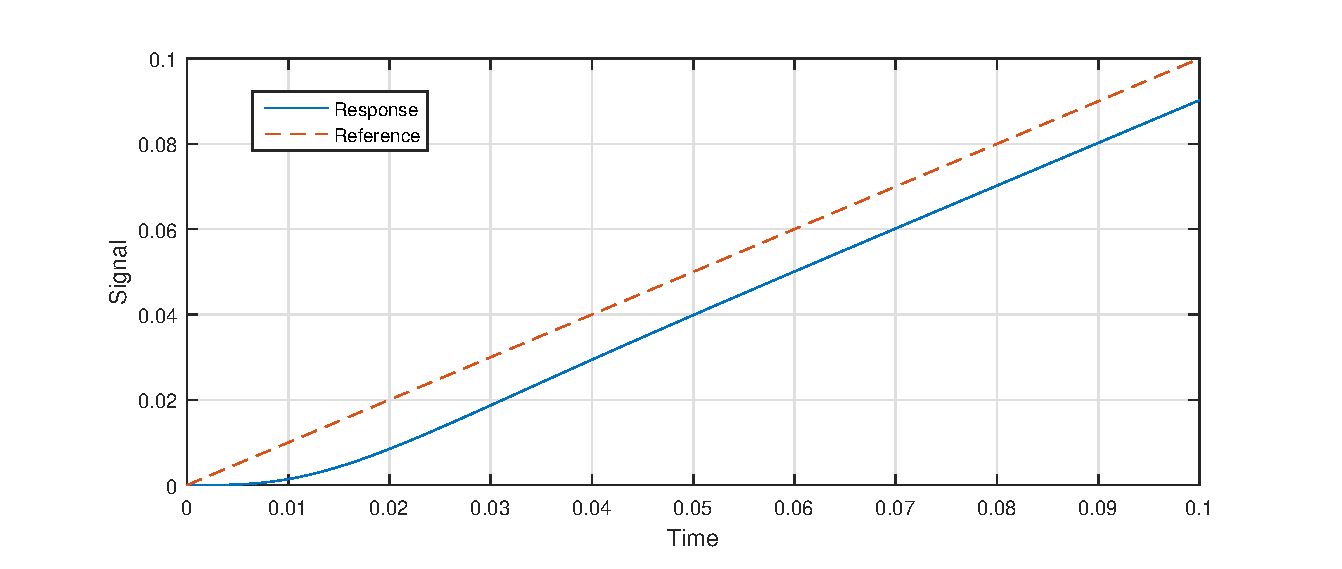
\includegraphics[width=\linewidth]{Plots/slope_delay1.eps}
  \end{center}
  \caption{System reaction under a slope signal.}
  \label{fig:slope}
\end{figure}

While overshoot and slope delay can only speak one aspect of the system, ISE is a rather comprehensive criterion. If reference signal is $r(t)$ and output of the closed loop system is $y(t)$, ISE is defined as $$ ISE = \int_{0}^{\tau} (r(t)-y(t))^2dt$$ where $\tau$ is the period of the signal if input is periodic. With such a layout, ISE constraint calls for transformation before it can be fitted into the context of GP. In \cite{malmquist2015tool} a method based on Fourier transform is used, in which a signal is at first decomposed as a series of harmonics and output of those harmonics can be calculated by checking the frequency response of the system. System reaction can be estimated by combining harmonic output together. Another approach use discretized state space model instead. Both methods can provide sufficient and precise information of the system reaction. In terms of efficiency, since the current software framework is running in Matlab and matrix is preferred in the software, state-space approach annihilate its counterpart. Therefore, the latter approach is illustrated here. In other context, harmonic approach might perform better instead.

The transfer function $G_{\text{cl}}(s)$ has all desired poles since it is  obtained by pole placement method. Suppose it is strictly proper and the transfer function is 
$$\frac{Y(s)}{R(s)}=G_{\text{cl}}(s)=\frac{b_1s^{n-1}+b_2s^{n-2}+ \cdots +b_n}{s^n+a_1s^{n-1}+ \cdots + a_n}=\frac{N_\text{cl}(s)}{D_{\text{cl}}(s)}$$ where $Y(s)$ and $R(s)$ are Laplace transform of output $y(t)$ and $r(t)$ respectively and $n \in \mathbf{N_{++}}$. Its state space model, by following the method from \cite{astrom2010feedback}, is given by 
\begin{equation}\label{eq:st_sp}
\begin{aligned} 
\dot{\mathbf{x}}&=A_{n \times n}\mathbf{x}+B_{n \times 1}r\\
y&=C_{1 \times n} \mathbf{x}
\end{aligned} 
\end{equation}
The state variable $\mathbf{x}$ is defined as $$\mathbf{x}=\left[\begin{array}{c}v^{(n)}\\ \vdots \\v^{(1)}\\v \end{array}\right]$$ where Laplace transform of $v$ fulfills $\sfrac{Y(s)}{V(s)}=N_{\text{cl}}(s)$ and $\sfrac{R(s)}{V(s)}=D_{\text{cl}}(s)$. The matrices of the model is given by $$ A_{n \times n} = 
 \left[\begin{array}{ccccc}
  -a_1 & -a_2 & \cdots & -a_{n-1} & -a_n \\
  1 &	0 & \cdots & 0 & 0 \\
  0 &	1 & \cdots & 0 & 0 \\
  \vdots  &   & \ddots & \vdots& \vdots  \\
  0 & 0 &  & 1 & 0
 \end{array}\right] $$ $$ B_{n \times 1} = \left[\begin{array}{c}1\\0\\ \vdots \\ 0 \end{array}\right]\; \text{and}\; C_{1 \times n} \left[\begin{array}{c}b_1\\b_2\\ \vdots \\ b_n \end{array}\right]^T $$
 
After discritizing the state space model, the whole trajectory can be expressed as a function of design variables and desired poles. Then ISE can be calculated based on trajectory.  